\section{Main Text}
    A document must be organized by three parts:
        \begin{enumerate}
            \item Introduction.
            \item Body.
            \item Conclusions.
        \end{enumerate}
    Remember that a paragraphs is an idea. Try to be clear, rigorous and concise.

\section{Work development}
    It is recommended to start this section with a global paragraph, which introduces the following subsections. About the content:
        \begin{itemize}
            \item Identify the objectives of the trial. Mention the standard and/or reference used to design the experiment.
            \item Consider that the tests seek the characterization of mechanical properties. Therefore, the selected mechanical properties must be justified to be obtained by the simulation.
            \item Whenever possible, look for references that contain experimental results.
            \item With all the above defined, choose the geometry to simulate. As far as possible, use the simplest geometry that allows obtaining the mechanical properties. The focus is the material, not the structure.
        \end{itemize}

    References must follow the following format: \textcite{Kalamkarov2006} (quote in text) or quote at the end of the sentence \citep{Kopac2005}. Book \citep{Mehta2014} and conference annals \citep{He2005a} they follow different formats. The reference must include the author, the title of the article or the book chapter, the year of publication, the name of the journal or publisher, etc. That is, all the information necessary for the reader to review the cited material.

\subsection{Description of the report}
    Images must contain text that describes them. The image should be clear enough so that it is understandable even without reading the article. The clarity and quality of the graphics are relevant to convey a message, so you have to avoid blurred images, with illegible or poor quality texts. This \LaTeX \ report supports images in formats in \verb|.pdf|, \verb|.jpeg| and \verb|.png|.

    Each image must be cited in the text, such as the \Cref{fig:my_label}

        \begin{figure}[htb]
            \centering
            \begin{subfigure}[t]{0.3\textwidth}
                \centering
                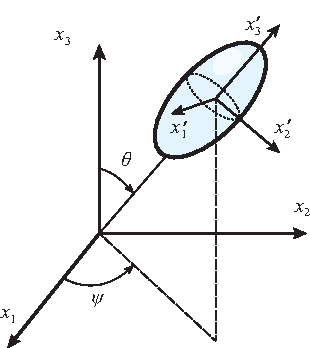
\includegraphics[]{figures/eulerang}
                \caption{Lorem ipsum}\label{fig:fig1}
            \end{subfigure}%
            ~
            \begin{subfigure}[t]{0.7\textwidth}
                \centering
                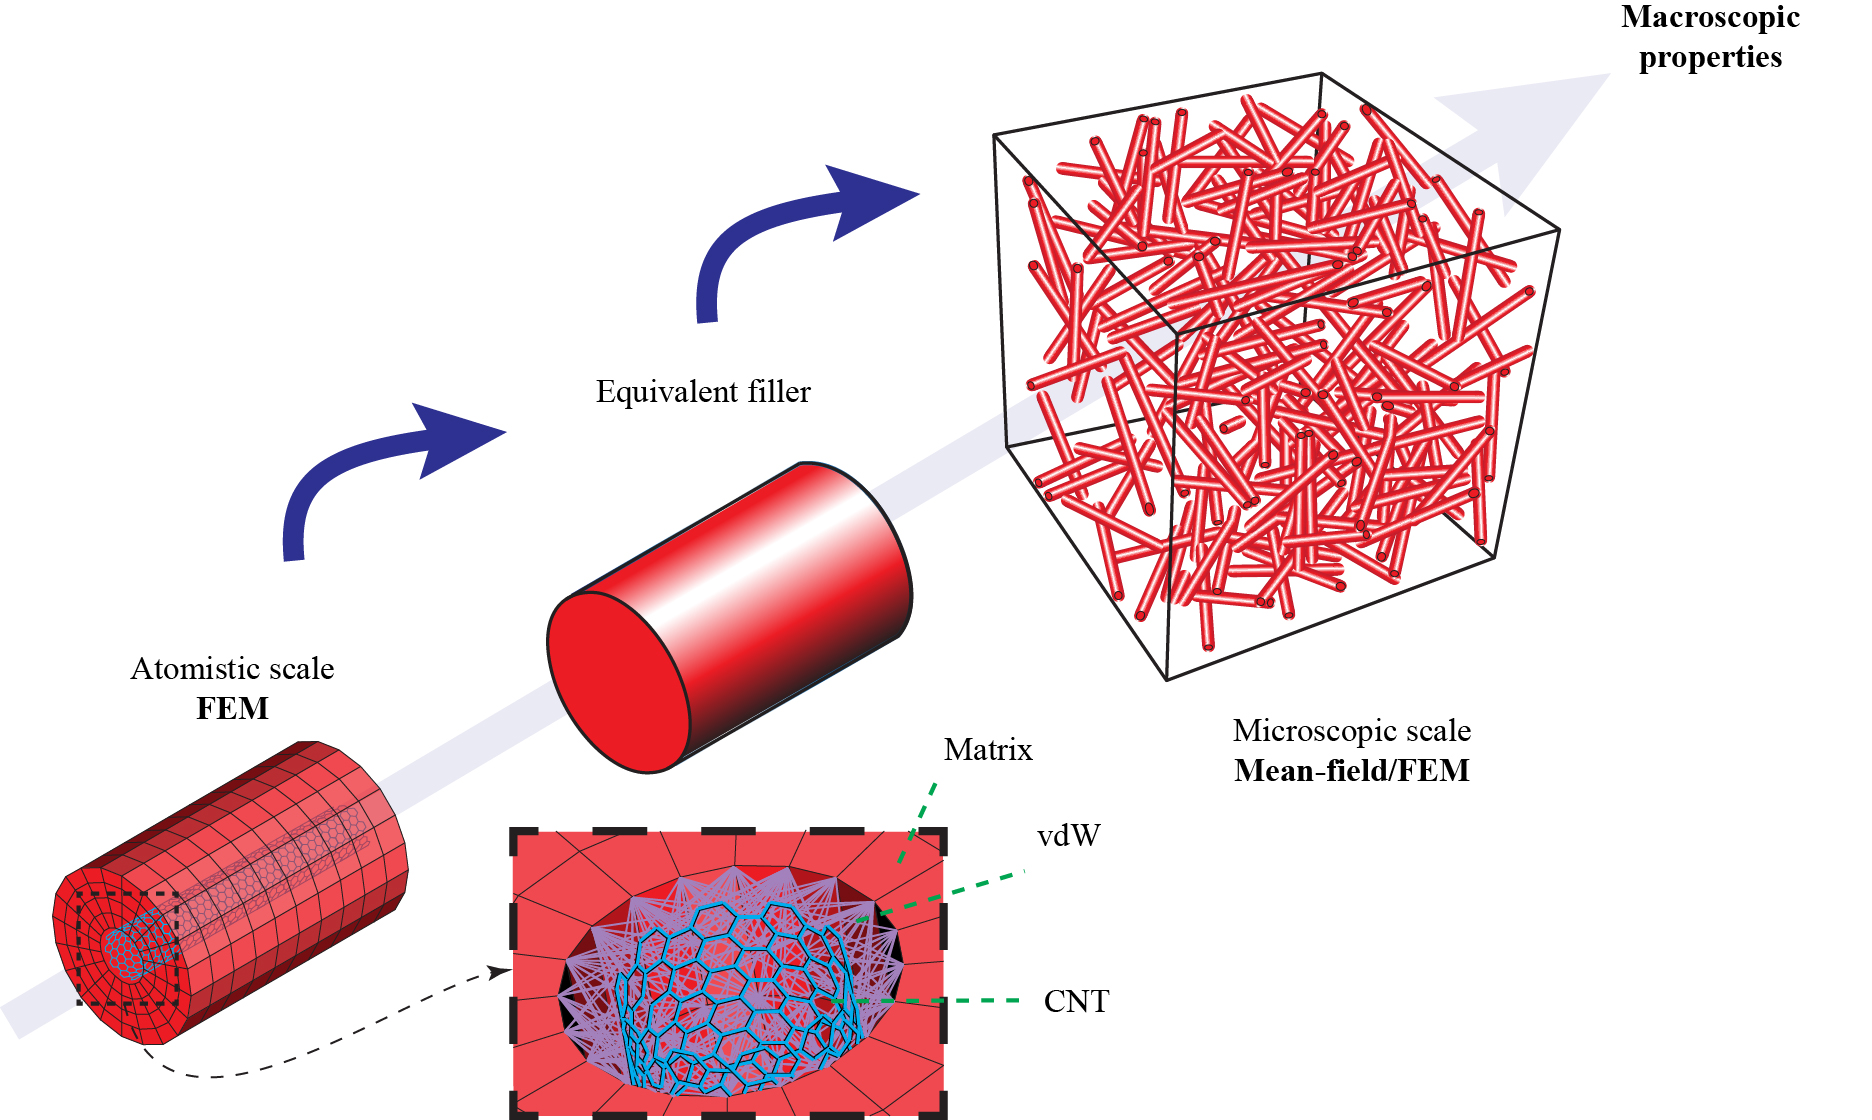
\includegraphics[scale=0.7]{figures/multiscale}
                \caption{Lorem ipsum}\label{fig:fig2}
            \end{subfigure}
            \caption{Caption \subref{fig:fig1} refered to left figure and \subref{fig:fig2} to refered to right figure.}
            \label{fig:my_label}
        \end{figure}

\subsection{Description of the simulations}
    It must include, in addition to its respective justification, the following:
        \begin{itemize}
            \item Software and version.
            \item Constitute law of material.
            \item Type of finite element.
            \item Total number of nodes and elements (for each type).
            \item Hypothesis on the behavior of the material (linear-elastic, bi-linear plasticity, perfectly plastic, etc.)
            \item Hypothesis on edge conditions (axisymmetry, plane deformation, 3D case).
        \end{itemize}
    The information provided must be such that it allows other researchers to reproduce the results.

    In the case of the mathematical notations and nomenclature for tensor is presented in \Cref{tab:generalnotation} (please note that some exceptions apply). An example of this and how to reference an equation is shown in the \Cref{eq:PK1}.

        \begin{table}[htbp]
            \caption{General scheme of notation.}
            \centering\begin{tabular}{ccc}\toprule
                Tensor order & Lagrangian & Eulerian \\\midrule
                Zero (scalar) & $m_0$      & $m$ \\
                1\textsuperscript{nd} (Vector) & \underbar{$X$}, $\bm{X}$, $X_i$ & \underbar{$x$}, $\bm{x}$, $x_i$ \\
                2\textsuperscript{nd} & \doubleunderline{$P$}, $\bm{P}$, $P_{ij}$ & \doubleunderline{$\sigma$}, $\bm{\sigma}$, $\sigma_{ij}$ \\
                3\textsuperscript{rd} & \multicolumn{2}{c}{$\mathcal{E}$, $E_{ijk}$} \\
                4\textsuperscript{th} & $\bm{\mathsf{C}}$, $C_{ijkl}$ & $\bm{\mathsf{c}}$, $c_{ijkl}$ \\\bottomrule
            \end{tabular}
            \label{tab:generalnotation}
        \end{table}

        \begin{equation}\label{eq:PK1}
            \bm{P}(\bm{F}) \coloneqq \frac{\partial W}{\partial \bm{F}}
        \end{equation}
        \nomenclature{$\Omega$}{Subset of a region occupied by a body}
        \nomenclature{$\partial\Omega$}{Boundary of a closed region $\Omega$}

\subsection{Results and analysis}
    For units of measure, use the \verb|siunitx| package. For example, \qty{1.0}{\kilogram} or \qty{100}{\giga\pascal} or $\rho = \qty{1490}{\kilogram\per\meter\cubed}$.
    The tables, like the images, must be cited in the text and must follow the format shown in the \Cref{tab:CLTresults}.

        \begin{table}[htbp]
            \centering
            \caption{Results of CLT buckling test, obtained from \textcite{pinaNumericalStudyElastic2019}.}
            \begin{tabular}{c
                            S[table-format=3.0]
                            S[table-format=2.0]
                            S[table-format=4.0]
                            S[table-format=2.2]
                            S[table-format=3.1]
                            S[table-format=3.2]
                            S[table-format=2.2]}
            \toprule
                {\multirow{2}{*}{\makecell{Test\\number}}}
                    & {\multirow{2}{*}{\makecell{Width\\/\unit{\milli\meter}}}} 
                        & {\multirow{2}{*}{\makecell{Total thickness\\/\unit{\milli\meter}}}}
                            & {\multirow{2}{*}{\makecell{Height\\/\unit{\milli\meter}}}}
                                & {\multirow{2}{*}{\makecell{$E$\\/\unit{\giga\pascal}}}}
                                    & {\multirow{2}{*}{\makecell{$\lambda_{eff}$}}}
                                        & {\multirow{2}{*}{\makecell{Critical load\\/\unit{\kilo\newton}}}}
                                            & {\multirow{2}{*}{\makecell{Critical stress\\/\unit{\mega\pascal}}}} \\
                &&&&&&&\\\midrule
            1.a   & 150   & 45    & 1000  & 11.65 & 87.8  & 71.85 & 10.64 \\
            1.b   & 150   & 45    & 1000  & 11.65 & 87.8  & 95.31 & 14.12 \\
            2.a   & 150   & 45    & 1980  & 11.65 & 164.6 & 35.76 & 5.3 \\
            2.b   & 150   & 45    & 1990  & 11.65 & 164.6 & 21.12 & 3.13 \\
            3.a   & 150   & 90    & 2000  & 11.29 & 83.1  & 210.14 & 15.57 \\
            3.b   & 150   & 90    & 2000  & 11.29 & 83.1  & 129.24 & 9.57 \\
            3.c   & 150   & 90    & 2000  & 11.29 & 83.1  & 168.98 & 12.52 \\
            3.d   & 150   & 90    & 2000  & 11.29 & 83.1  & 194.89 & 14.44 \\\bottomrule
            \end{tabular}%
            \label{tab:CLTresults}%
        \end{table}%

\section{Conclusions and perspectives}
    The conclusions interpret the results towards a concise recommendation. The perspective establishes a broader point of view on the conclusions, establishing possible lines of development around the conclusions of the work.